\part{Les données}
    \chapter{Le périmètre produit}
    \label{perimetre_produit}
        \section{Accessibilité de la donnée en fonction des branches}

        Comme vu à la section \mref{outils_infos}, les systèmes d'information associés à la gestion de l'information produit offrent des niveaux d'accès hétérogènes à la donnée produit.
        Le récapitulatif par branche est le suivant : 
        \begin{description}
            \item[\'{E}piSaveurs :] on peut simplement accéder à l'ensemble des données produit, structurées, non structurées (i.e. textes longs) et pièces jointes
            \item[PassionFroid :] on a uniquement la possibilité d'exporter manuellement les données structurées articles depuis le système de gestion SAP.
            Elles permettent de produire quelques analyses quantitatives.
            Il est difficile de faire des exports en masse de l'outil de gestion de l'information produit GIP (cf. section \mref{GIP}).
            \item[TerreAzur :] idem PassionFroid, si ce n'est qu'en plus le système GIP n'est pas utilisé au sein de cette branche.
            \item[Délice et Création :] le système d'information ne permet pas d'exporter les données et donc de produire des indicateurs détaillés. On peut toutefois avoir des informations quantitatives de la part des opérationnels.
            \item[Saveurs d'Antoine :] idem Délice et Création
            \item[Pomona Suisse :] la branche est en cours de structuration, et les référentiels articles ne sont pas partagés entre les succursales. Il n'est pas possible d'obtenir d'information quantitative sur ces données.
            \item[Pomona Iberia :] idem Pomona Suisse
        \end{description}

        Pour les analyses quantitatives, on pourra se baser sur des extractions uniquement pour les branches RHD (\'{E}piSaveurs, PassionFroid, TerreAzur).
        L'ensemble des analyses portant sur les branches RHD sont produites sur la base d'extractions de leur système de gestion SAP.

        \section{Analyses quantitatives}

        Les graphes de cette section ont été produits via le code présenté en annexe, au chapitre \mref{code:analyse_quantitative}.
        Les données pour les branches spécialistes (Délice et Création et Saveurs d'Antoine) sont issues d'informations fournies par le métier, hors système.
        Dans l'ensemble de cette section, on raisonnera à la maille \emph{article} (cf. la définition article vs. produits, présentée à la section \mref{produit_article}).

            \subsection{Comparatifs entre les branches}

                En termes de volumétrie article (cf. \reffig{fig:volumetrie_article}, c'est TerreAzur qui possède le référentiel le plus étendu (environ 62 000 articles de marchandises actifs).
                Cela s'explique par le fait que cette branche commercialise essentiellement des produits bruts, non-préemballés (ex : des cagettes de fruits ou de légumes).
                Or, ces produits ne sont pas clairement identifiés, par exemple par un GTIN.
                Au démarrage de cette branche, afin de limiter la charge sur les gestionnaires de référentiels, le parti a été pris de créer en avance de phase l'ensemble des articles susceptibles d'être commercialisés.
                Cela s'est traduit par la création d'un grand nombre d'articles, du fait de l'application \og brutale \fg de la combinatoire des différents critères pouvant définir un produit.
                Un exemple (fictif) serait, sur les pommes : 
                \begin{itemize}
                    \item 8 variétés possibles (Gala, Golden, \dots)
                    \item 4 calibres possibles
                    \item 6 conditionnements possibles (plateau 6kg, plateau 4,5kg, \dots)
                    \item 2 catégories (I, II)
                    \item 8 origines (France, Espagne, \dots)
                \end{itemize}
                ce qui donne un total de 3072 articles uniquement sur cette gamme de produits.

                Viennent ensuite PassionFroid, et \'{E}piSaveurs, qui sont les autres \og grosses \fg branches historiques du Groupe.

                \begin{figure}[htbp]\CenterFloatBoxes
                    \begin{floatrow}
                    \ffigbox{%
                        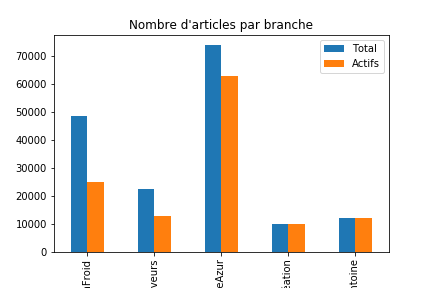
\includegraphics[width=200pt]{img/Articles par branche.png}%
                    }{%
                      \caption{Volumétrie article par branche}%
                      \label{fig:volumetrie_article}%
                    }
                    \capbtabbox[][][c]{%
                        \begin{tabular}{lccc}
\toprule
{} &  Total &  Actifs &  Marchandises \\
\textbf{Branche           } &        &         &               \\
\midrule
\textbf{PassionFroid      } &  48478 &   24898 &         24554 \\
\textbf{EpiSaveurs        } &  22498 &   12798 &         12241 \\
\textbf{TerreAzur         } &  73804 &   62789 &         62710 \\
\textbf{Délice et Création} &  10000 &       - &             - \\
\textbf{Saveurs d'Antoine } &  12000 &       - &             - \\
\bottomrule
\end{tabular}
%
                    }{%
                      \caption{Volumétrie article par branche}%
                    }
                    \end{floatrow}
                \end{figure}
                    
                Une analyse du recouvrement des référentiels montre que dans l'ensemble, les branches ne travaillent pas les mêmes articles (cf. \reffig{fig:venn_article}).
                PassionFroid commercialise certains produits des branches \'{E}piSaveurs et TerreAzur, mais cela s'explique par une petite entité luxembourgeoise qui travaille des produits de tout type de stockage.
                Une réserve toutefois par rapport à cette analyse de recouvrement produit : elle sous-estime vraisemblablement lesdits recouvrements, dans la mesure où la présence de doublons n'est pas prise en compte.

                \begin{figure}[htbp]
                    \begin{center}
                    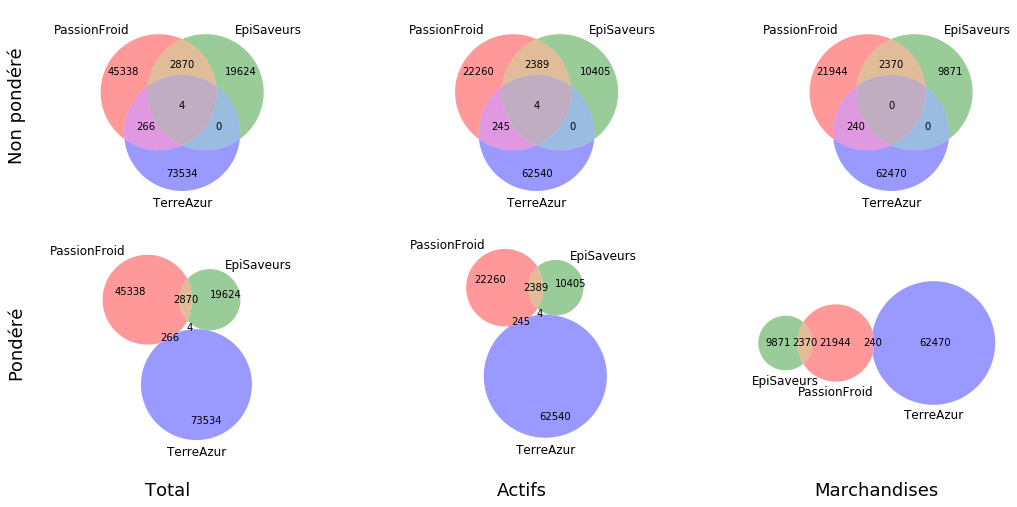
\includegraphics[width=\linewidth]{img/Diagrammes de Venn articles.png}
                    \end{center}
                    \caption{Recouvrements entre branches RHD}
                    \label{fig:venn_article}
                \end{figure}       

            \subsection{Les grands types de produits}

            Comme montré à la \reffig{fig:repart_art_categ}, on voit bien (en plus du fait que les articles étaient peu partagés entre les branches) que : 
            \begin{itemize}
                \item les deux types d'articles (négoce et presté) sont utilisés par les 3 branches
                \item c'est tout de même PassionFroid qui fait l'utilisation majoritaire d'articles prestés
                \item les branches \emph{ne} partagent \emph{pas} l'utilisation des autres \og catégories \fg\ (groupe de marchandises, conditions de stockage, hiérarchie produit, \dots)
            \end{itemize}
            Les indicateurs sont également récapitulés dans la \reftable{tab:repart_art_categ}.

            \begin{figure}[htbp]
                \begin{center}
                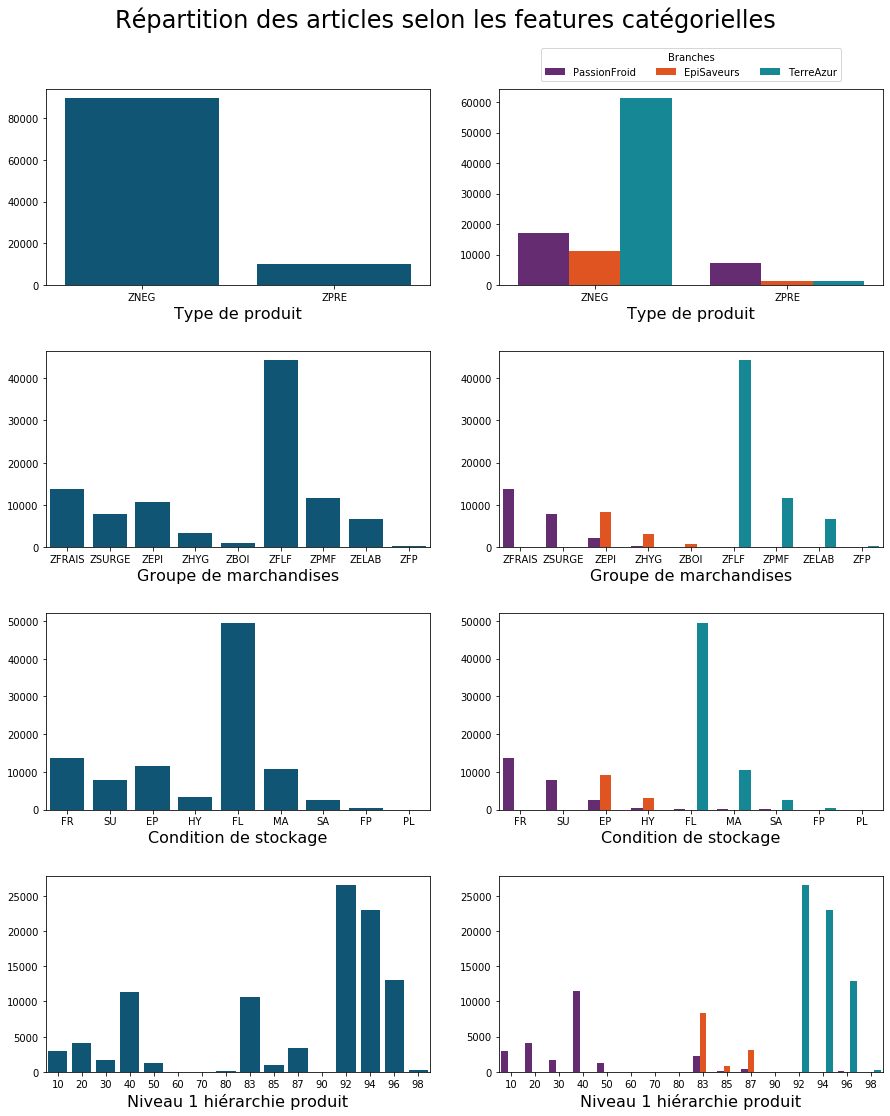
\includegraphics[width=\linewidth]{img/Repartition articles categories.png}
                \end{center}
                \caption{Répartition des articles en fonction des variable catégorielles}
                \label{fig:repart_art_categ}
            \end{figure}

            \begin{table}[htbp]
                \footnotesize
                \begin{center}
                \begin{tabular}{lccc}
\toprule
\textbf{Branche} &  PassionFroid &  EpiSaveurs &  TerreAzur \\
\textbf{Type de produit             } &               &             &            \\
\midrule
\textbf{ZNEG - Article de négoce    } &         17166 &       11048 &      61273 \\
\textbf{ZPRE - Article de prestation} &          7388 &        1193 &       1437 \\
\bottomrule
\end{tabular}

                \vspace{5pt}
                \begin{tabular}{lccc}
\toprule
\textbf{Branche} & PassionFroid & EpiSaveurs & TerreAzur \\
\textbf{Groupe de marchandises   } &              &            &           \\
\midrule
\textbf{ZSURGE - Surgelés        } &         7756 &          - &         - \\
\textbf{ZFRAIS - Frais           } &        13785 &          6 &         4 \\
\textbf{ZEPI - Epicerie          } &         2298 &       8305 &         - \\
\textbf{ZBOI - Boissons          } &          126 &        826 &         - \\
\textbf{ZHYG - Hygiène           } &          350 &       3078 &         - \\
\textbf{ZFLF - Fruits et Légumes } &            4 &          - &     44133 \\
\textbf{ZPMF - Produits de la mer} &          142 &          - &     11594 \\
\textbf{ZELAB - Produits élaborés} &           91 &          - &      6644 \\
\textbf{ZFP - Fleurs et plantes  } &            - &          - &       297 \\
\textbf{ZAUTRE - Autres          } &            2 &         26 &        38 \\
\bottomrule
\end{tabular}

                \vspace{5pt}
                \begin{tabular}{lcccc}
\toprule
\textbf{Branche} & PassionFroid & EpiSaveurs & TerreAzur &  Total \\
\textbf{Condition de stockage } &              &            &           &        \\
\midrule
\textbf{SU - Surgelés         } &         7758 &          - &         - &   7758 \\
\textbf{FR - Frais            } &        13781 &          6 &         3 &  13790 \\
\textbf{EP - Epicerie         } &         2430 &       9155 &         - &  11585 \\
\textbf{HY - Hygiène          } &          344 &       3080 &         - &   3424 \\
\textbf{FL - Fruits et légumes} &           78 &          - &     49508 &  49586 \\
\textbf{MA - Marée            } &          126 &          - &     10501 &  10627 \\
\textbf{FP - Fleurs et plantes} &            - &          - &       286 &    286 \\
\textbf{SA - Saurisserie      } &           34 &          - &      2408 &   2442 \\
\textbf{PL - Publicié         } &            2 &          - &         1 &      3 \\
\bottomrule
\end{tabular}

                \vspace{5pt}
                \begin{tabular}{lccc}
\toprule
\textbf{Branche} & PassionFroid & EpiSaveurs & TerreAzur \\
\textbf{Niveau 1 hiérarchie produit        } &              &            &           \\
\midrule
\textbf{10 - Beurre, oeufs, fromage        } &         3010 &          6 &         1 \\
\textbf{20 - Elaborés                      } &         4150 &          2 &         6 \\
\textbf{30 - Garnitures et fruits          } &         1701 &          - &         - \\
\textbf{40 - Produits carnés               } &        11413 &          - &         - \\
\textbf{50 - Produits de la mer            } &         1214 &          - &         2 \\
\textbf{60 - Consommables                  } &            1 &          - &         - \\
\textbf{70 - Emballage                     } &            - &          1 &         - \\
\textbf{80 - Publicité sur le lieu de vente} &           34 &         25 &        37 \\
\textbf{83 - Epicerie                      } &         2306 &       8296 &         - \\
\textbf{85 - Liquides                      } &          135 &        836 &         - \\
\textbf{87 - Hygiène et entretien          } &          348 &       3075 &         - \\
\textbf{90 - Services                      } &           10 &          - &         - \\
\textbf{92 - Fruits                        } &           35 &          - &     26543 \\
\textbf{94 - Légumes                       } &           37 &          - &     22929 \\
\textbf{96 - Produits de la mer Frais      } &          160 &          - &     12891 \\
\textbf{98 - Fleurs - plantes              } &            - &          - &       301 \\
\bottomrule
\end{tabular}

                \end{center}
                \caption{Utilisation des variables catégorielles article au sein des branches RHD}
                \label{tab:repart_art_categ}
                \normalsize
            \end{table}

            Possibilité d'extension: 
            - ajouter la vision produit (via les FIA)
            - faire une sorte d'heatmap qui montre la forte correlation entre les différentes variables catégorielles (et les définitions associées. Ex: ZELAB + SA = Saurisserie, etc...)

    \chapter{Les données utilisables, issues du PIM}
        \large
        Comme vu au chapitre \mref{perimetre_produit}, les données produit ne sont simplement accessibles que pour la branche \'{E}piSaveurs.
        On se focalisera donc sur cette branche pour la suite de cette étude, ainsi que sur les produits alimentaires (en excluant donc les produits d'hygiène et de chimie, cf. section \mref{produits_nonal}).
        Contrairement au chapitre précédent, ici on travaillera à la maille \emph{produit} (cf. la distinction produit vs. article section \mref{produit_article}).
        L'ensemble des tableaux et graphes de ce chapitre ont été produit via le notebook "Analyse des données du PIM", présenté en annexe \mref{code:analyse_donnees_PIM}.
        \normalsize

        \section{Données structurées}

            \subsection{Description des données structurées}

        Les données dites structurées sont l'ensemble des données qui peuvent prendre leurs valeurs dans un domaine restreint.
        Par exemple, ce sont les données booléennes, les choix issus de listes déroulantes, les valeurs numériques\dots
        Les principales données structurées pour les produits alimentaires dans le PIM sont : 
        \begin{description}
            \item[le code du produit :] calculé par le système
            \item[le fournisseur :] référence croisée vers le code du fournisseur
            \item[le type de produit :] épicerie, boisson alcoolisée, hygiène, chimie, boisson non-alcoolisée
            \item[le GTIN du produit :] identifiant numérique unique, utilisé entre autres pour l'étiquetage sous forme de code à barres~\cite{GS1_GTIN}
            \item[le type d'unité de base :] paquet, boîte, sachet, rouleau, bouteille, pot, \dots
            \item[les poids :] brut, net, net égoutté (pour les conserves)
            \item[le volume :] pour les produits liquides
            \item[les durées de vie :] le type (Date Limite de Consommation ou Date de Durabilité Minimale) et la durée (totale à fin de production, garantie à livraison)
            \item[les modes de conservation avant/après ouverture :] à température ambiante, au réfrigérateur puis à consommer sous 2 jours, \dots
            \item[les labels :] le(s) label(s) s'appliquant au produit (cf. section \ref{labels} page \pageref{labels})
            \item[les régimes particuliers :] Halal, Casher, Sans porc, Végétarien, Végétalien, \dots
            \item[les caractéristiques spéciales :] sans OGM, non traité par ionisation
            \item[la présence d'allergènes :] le niveau de présence de chacun des 14 allergènes réglementés (cf. section \mref{composition}) : absence, présence ou traces
            \item[les matières grasses utilisées :] palme, beurre, coco, tournesol, palmiste, \dots
            \item[les additifs présents :] les codes Exxx et les fonctions des additifs mis en oeuvre~\cite{additifs_regl_eu}\cite{additifs_wiki}
            \item[les données nutritionnelles obligatoires :] pour 100g ou 100mL, valeur énergétique (en kJ et kcal), matières grasses, dont acides gras saturés, Glucides, dont sucres simples, Fibres, Protéines, simplement
            \item[les données nutritionnelles facultatives :] vitamines, minéraux, omégas, \dots
            \item[les allégations nutritionnelles :] riche en, faible en, sans,\dots associé à un nutriment défini dans les 2 points précédents
            \item[le nutriscore :] note allant de A à E, définie dans la loi Santé de janvier 2016
            \item[le taux de TVA :] un des quatre taux définis dans la réglementation française
            \item[le code nomenclature douanière :] code identifiant les marchandises défini par les douanes pour la Déclaration d'\'{E}change de Biens~\cite{notions_DEB}
            \item[le pays d'origine pour la DEB :] le pays d'origine à déclarer dans la Déclaration d'\'{E}change de Biens~\cite{notions_DEB}
            \item[les informations logistiques :] il s'agit du plan de conditionnement et de palettisation du produit. Elles regroupent les différents niveaux et les quantités pour passer de l'un à l'autre (ex : 3 boites dans un cartons, 64 cartons dans une palette), les poids et dimensions de ces niveaux logistiques, leurs GTIN, \dots
        \end{description}
        
            \subsection{Analyse de ces données structurées}

                \subsubsection{Données d'identification}
                Un exemple et une description statistique de ces données est présentées aux \reftable{tbl:exemple_idt} et \reftable{tbl:desc_idt}.
                On peut en tirer les conclusions suivantes : 
                \begin{itemize}
                    \item Les codes produits sont bien des identifiants uniques des produits : on a autant de valeurs uniques que de valeurs renseignées
                    \item Une proportion importante de produits (91\%) porte un GTIN (cf. \cite{GS1_GTIN}), ce qui reflète une \og maturité \fg des filières produits avec lesquelles travaille \'{E}piSaveurs.
                    \item Ces GTIN sont également censés être des identifiants uniques des produits. Néanmoins, comme présenté à la 
                \end{itemize}

                \begin{figure}[htbp]\CenterFloatBoxes
                    \begin{floatrow}
                    \ffigbox{%
                        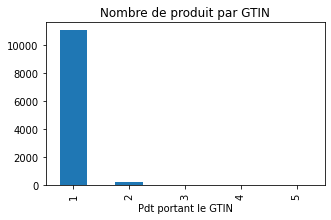
\includegraphics[width=200pt]{img/repartition_gtin.png}%
                    }{%
                      \caption{Nombre de produits par GTIN}%
                      \label{fig:produit_par_GTIN}%
                    }
                    \capbtabbox[][][c]{%
                        \begin{tabularx}{\linewidth}{lX}
\toprule
{} &  Nb de GTIN \\
\textbf{Pdt portant le GTIN} &             \\
\midrule
\textbf{1                  } &       11068 \\
\textbf{2                  } &         227 \\
\textbf{3                  } &          22 \\
\textbf{4                  } &          20 \\
\textbf{5                  } &           1 \\
\bottomrule
\end{tabularx}
%
                    }{%
                      \caption{Nombre de produits par GTIN}%
                    }
                    \end{floatrow}
                \end{figure}        


        TODO : continuer l'analyse par domaine de données.

        
        \begin{landscape}   
            \begin{table}
                \RawFloats
                {\scriptsize
                \begin{center}
                \begin{tabular}{lcccc}
\toprule
{} &     Code produit & Code fournisseur & Type de produit &            GTIN \\
\textbf{uid                                 } &                  &                  &                 &                 \\
\midrule
\textbf{1c6a9d67-8fea-4b5e-a0c3-29f9338e1128} &  PIMP-0000004399 &  PIMF-0000000112 &  alcoholicDrink &   3080210001100 \\
\textbf{07d045b6-4cde-403d-b577-a11b899dcd29} &  PIMP-0000005503 &  PIMF-0000000060 &         grocery &   3760128846009 \\
\textbf{40b933d8-d8eb-4867-8d14-83fc999c5281} &  PIMP-0000010837 &  PIMF-0000000011 &         grocery &  13274643110097 \\
\textbf{ae72ae63-7b12-4bcf-b15e-52acff941375} &  PIMP-0000003913 &  PIMF-0000000283 &         hygiene &   3342690094301 \\
\textbf{81ed6169-03eb-44b5-a3eb-8a25e879948e} &  PIMP-0000010172 &  PIMF-0000000178 &         hygiene &            None \\
\bottomrule
\end{tabular}
%
                \caption{Exemples de codes d'identification}%
                \label{tbl:exemple_idt}%
                \bigskip\bigskip
                \begin{tabularx}{\linewidth}{lXXXX}
\toprule
{} &     Code produit & Code fournisseur & Type de produit &   GTIN \\
\midrule
\textbf{count } &            13183 &            13183 &           13183 &  12019 \\
\textbf{unique} &            13183 &              605 &               5 &  11333 \\
\textbf{top   } &  PIMP-0000011105 &  PIMF-0000000179 &         grocery &        \\
\textbf{freq  } &                1 &              370 &            8755 &    352 \\
\bottomrule
\end{tabularx}
%
                \caption{Description des codes d'identification sur le dataframe}%
                \label{tbl:desc_idt}%   
                \end{center}
                }
            \end{table}

            \begin{table}
                \RawFloats
                {\scriptsize
                \begin{center}
                \begin{tabularx}{\linewidth}{lXXXXX}
\toprule
{} & Unité de base &  Poids net &  Poids brut &  Poids net égoutté &  Volume \\
\textbf{uid                                 } &               &            &             &                    &         \\
\midrule
\textbf{4bf17478-a4fd-43b3-9920-151f73b76ba0} &           COL &      1.260 &       1.700 &                  - &       - \\
\textbf{af78f096-2406-48a4-8481-d461d6b32bb0} &           COL &      1.200 &       1.560 &                  - &       - \\
\textbf{855fcaf4-81c8-4f46-8e99-101202f07e0b} &           SAC &      1.000 &       1.040 &                  - &       - \\
\textbf{d092afe5-e0fe-42d8-ba58-dc2e9b579767} &           BTE &      0.340 &       0.360 &                  - &    0.33 \\
\textbf{995ef7a8-8d7c-4d93-9528-517ebbd60f67} &           SAC &      0.295 &       0.297 &                  - &       - \\
\bottomrule
\end{tabularx}
%
                \caption{Exemples de dimensions}%
                \label{tbl:exemple_dim}%
                \bigskip\bigskip
                \begin{tabular}{lccccc}
\toprule
{} & Unité de base &  Poids net &  Poids brut &  Poids net égoutté &    Volume \\
\midrule
\textbf{count } &         13183 &  12817.000 &   12817.000 &           1026.000 &  1911.000 \\
\textbf{unique} &            30 &          - &           - &                  - &         - \\
\textbf{top   } &           BTE &          - &           - &                  - &         - \\
\textbf{freq  } &          3051 &          - &           - &                  - &         - \\
\textbf{mean  } &             - &      3.111 &       2.985 &              1.475 &     7.751 \\
\textbf{std   } &             - &     59.623 &      42.187 &              1.133 &    78.979 \\
\textbf{min   } &             - &      0.000 &       0.000 &              0.000 &     0.000 \\
\textbf{25\%   } &             - &      0.482 &       0.535 &              0.480 &     0.500 \\
\textbf{50\%   } &             - &      1.000 &       1.100 &              1.500 &     0.900 \\
\textbf{75\%   } &             - &      3.000 &       3.291 &              2.380 &     2.500 \\
\textbf{max   } &             - &   4900.000 &    4730.500 &             10.000 &  3100.000 \\
\bottomrule
\end{tabular}
%
                \caption{Description des dimensions sur le dataframe}%
                \label{tbl:desc_dim}%  
                \end{center}
                }
            \end{table}

            \begin{table}
                \RawFloats
                {\scriptsize
                \begin{center}
                \begin{tabularx}{\linewidth}{lXXXXXXX}
\toprule
{} &  Durée de vie totale &  Durée minimale restante & Type de conservation & Conservation avant ouv. & Convervation après ouv. & Température &  data\_ok \\
\textbf{uid                                 } &                      &                          &                      &                         &                         &             &          \\
\midrule
\textbf{61908e4e-4f95-4e69-b04a-2203b5e68a84} &                 28.0 &                     18.0 &                   AM &      ambientTemperature &         coolAndDryPlace &           - &    False \\
\textbf{f254910f-8562-431e-a499-cae5e67158b7} &                540.0 &                    360.0 &                   AM &      ambientTemperature &         coolAndDryPlace &           - &     True \\
\textbf{cfbf9793-4e5f-48e7-8dc0-d7653fe47d70} &                 24.0 &                     15.0 &                   AM &         coolAndDryPlace &         coolAndDryPlace &           - &    False \\
\textbf{e165da13-1f8b-4a2f-9271-fc507e571cbb} &                    - &                        - &                   AM &                       - &                       - &           - &    False \\
\textbf{8c764293-ba0a-4103-8465-23a4f5eff7bb} &                360.0 &                    240.0 &                   AM &      ambientTemperature &            notConcerned &           - &    False \\
\bottomrule
\end{tabularx}
%
                \caption{Exemples de conservation}%
                \label{tbl:exemple_cons}%
                \bigskip\bigskip
                \begin{tabularx}{\linewidth}{lXXXXXX}
\toprule
{} &  Durée de vie totale &  Durée minimale restante & Type de conservation & Conservation avant ouv. & Convervation après ouv. & Température \\
\midrule
\textbf{count } &             8946.000 &                 9466.000 &                12806 &                    9977 &                    9947 &          21 \\
\textbf{unique} &                    - &                        - &                    2 &                       7 &                      18 &           9 \\
\textbf{top   } &                    - &                        - &                   AM &      ambientTemperature &         coolAndDryPlace &          15 \\
\textbf{freq  } &                    - &                        - &                12772 &                    8270 &                    4512 &           6 \\
\textbf{mean  } &              651.406 &                  351.618 &                    - &                       - &                       - &           - \\
\textbf{std   } &              487.412 &                  380.255 &                    - &                       - &                       - &           - \\
\textbf{min   } &                0.000 &                    0.000 &                    - &                       - &                       - &           - \\
\textbf{25\%   } &              360.000 &                  180.000 &                    - &                       - &                       - &           - \\
\textbf{50\%   } &              540.000 &                  300.000 &                    - &                       - &                       - &           - \\
\textbf{75\%   } &              900.000 &                  480.000 &                    - &                       - &                       - &           - \\
\textbf{max   } &             9999.000 &                 9999.000 &                    - &                       - &                       - &           - \\
\bottomrule
\end{tabularx}
%
                \caption{Description des conservations sur le dataframe}%
                \label{tbl:desc_cons}%  
                \end{center}
                }
            \end{table}

        \normalsize
        \end{landscape}


        \section{Données non structurées}
        
            \subsection{Les libellés}

            Plusieurs libellés permettent de faire référence à chaque produit, avec des usages distincts:
            \begin{description}
                \item[Libellé temporaire unité de besoin :] il s'agit simplement d'un libellé qui est choisi par la personne à l'origine de la demande de référencement produit (souvent l'acheteur, cf. \reffig{fig:processus_article}), afin que le fournisseur comprenne sur quel produit porte le référencement.
                \item[Désignation du produit fournisseur :] c'est le libellé qui est donné par le fournisseur afin d'identifier simplement son produit.
                \item[Code article interne fournisseur :] c'est l'identifiant du produit, dans le système de gestion du fournisseur. Il s'agit généralement de codes, avec autant de formats distincts que de fournisseur venant contribuer.
                \item[Marque commerciale du produit :] il s'agit du nom de la marque commerciale du produit. 
                \item[Dénomination réglementaire :] c'est le libellé qui doit décrire de manière neutre le produit, sans notion liée au marketing (telle que la marque, entre autres), et qui doit obligatoirement figurer sur l'emballage du produit.
            \end{description}

            Ajouter ici quelques exemples issus du PIM sur ces libellés.

            \subsection{Les listes d'ingrédients}
            
            L'autre grand type de donnée non structurées sont les listes d'ingrédients.
            La construction des listes d'ingrédients doit suivre les règles suivantes, même si l'application n'est pas toujours parfaitement respectée :
            \begin{itemize}
                \item elle doit détailler l'ensemble des ingrédients, y compris les additifs et les arômes
                \item elle doit être triée par ordre d'importance pondérale décroissante (i.e. les ingrédients les plus représentatifs en poids doivent être cités en premier)
                \item la quantité de certains ingrédients (en pourcentage de la masse) par exemple ceux mis en valeur sur l'étiquetage ou dans la dénomination de vente (ex. gâteau aux fraises, pizza au jambon)
            \end{itemize}
            Même s'il ne s'agit pas d'une exigence réglementaire, le Groupe Pomona demande à ses fournisseurs de ne pas distinguer les ingrédients par phase comme cela se fait parfois.
            Cela signifie, par exemple, séparer une partie de la composition du produit (la pâte de la garniture pour une tarte, la sauce et les raviolis, \dots).
            De telles pratiques peuvent parfois induire le consommateur en erreur, comme par exemple dans la liste d'ingrédients suivante (s'applique à des chips de légumes):
            \begin{quotation}
                Légumes 64\% (betterave, panais, carottes, patates douces), huile de tournesol, sel marin.
            \end{quotation}
            Sans l'artifice d'avoir regroupé les légumes en une seule phase, le premier ingrédient de la liste aurait pu être l'huile de tournesol, qui est un ingrédient moins attractif pour un consommateur de chips de légumes.

            \emphbox{
            Les contraintes ci-dessus s'appliquant aux listes d'ingrédients font qu'en général, il s'agit d'une énumération d'ingrédients, sans doublon.
            }

            Fous-y des exemples ici aussi.

        \section{Pièces jointes}
            \label{pieces_jointes}

            Dans chacune des sections, mentionner la volumétrie de données accessibles (avec les facettes migration, statuts, \& compagnie) et tout

            \subsection{Fiches techniques fournisseur}
            \subsection{\'{E}tiquettes produit}
            \subsection{Fiches logistiques fournisseur}
            \subsection{Fiches techniques et argumentaires Pomona}
        \section{Récapitulatif de la complétude des données}

        Mettre ici un ou plusieurs tableaux récapitulatifs illustrant les données possédées quantitativement.

        \section{Analyse qualitative des données}
        
        Montrer qu'un sondage basique fait que la qualité actuelle est perfectible

        Mettre également la distribution numérique des produits par fournisseur et insister sur la difficulté posée par de multiples formats

        Dire ici qu'il y a finalement beaucoup de pdf qui possèdent des textes extractibles vs. uniquement des images.

        \section{Les données \og manuellement étiquetées \fg}

        Montrer comment elles ont été produites

        Expliciter les règles de gestion qui ont été listées pendant l'étiquetage manuel

        Evaluer la cohérence entre étiquettes manuelles et contenu du PIM
